% -*- root: main.tex -*-

\chapter{Modelowanie obiektowe dla Cassandry}

Na podstawie wyników wydajnościowych przedstawionych w~sekcji~\ref{sec:cassandra_orm_performance_summary} Autor zaproponował odmienną koncepcję mechanizmu mapowania obiektowego dla bazy danych Cassandra. Aby uwypuklić różnice pomiędzy przedstawioną propozycją i~tradycyjnymi mechanizmami ORM Autor postuluje stosowanie odmiennego nazewnictwa. Omówiona w~sekcji~\ref{sec:om_for_cassandra_concept} koncepcja, która będzie rozwijana w~dalszej części pracy, nazywana będzie \textbf{modelowaniem obiektowym}:

\begin{itemize}
	\item Mechanizmy mapowania obiektowo-relacyjnego nie wymuszają na użytkowniku kolejności projektowania komponentów. Osiągalne są zarówno podejście \emph{code first}\footnote{Code first (ang. dosłownie ,,najpierw kod źródłowy'') - w~kontekście ORM oznacza to modelowanie dziedziny za pomocą kodu źródłowego, z~którego następnie generowany jest schemat bazy danych.}, jak i~\emph{database first}\footnote{Database first (ang. dosłownie ,,najpierw baza danych'') - w~kontekście ORM oznacza to modelowanie dziedziny jako schemat bazodanowy, do którego następnie pisany jest mapujący kod źródłowy.}. W~proponowanym przez Autora modelowaniu obiektowym, ze względu na występowanie struktur wysokiego poziomu odpowiadających wzorcom projektowym, podejście \emph{database first} jest możliwe tylko teoretycznie lub w~bardzo ograniczonym zakresie. Znacznie bardziej efektywne jest podejście \emph{code first}. Posiada ono wsparcie implementacyjne - generację schematu - i~jest rekomendowane przez Autora.
	\item W~mechanizmach mapowania obiektowo-relacyjnego mapowanie odpowiada najczęściej typom danych, natomiast w~obrębie danego typu jest ono jednoznaczne. Przykładowo identyfikator konwertowany jest na liczbowy klucz główny, lista przechowywana jest jako relacja, a~ciąg znaków przekształcany jest na typ \emph{VARCHAR}. W~przypadku modelowania obiektowego dla Cassandry wybór wyznaczać będzie natomiast sposób przechowywania danej wartości. W~zależności od narzuconego sposobu modelowania listy będzie mogła zostać ona zrzutowana na wartość kolumny o~typie \verb+list+, nazwy kolumn w~wierszu lub osobną tabelę.
	\item Mapowanie obiektowo-relacyjne dostarcza przede wszystkim niskopoziomowe odpowiedniki typów bazodanowych. Wyjątkiem jest relacja wiele-do-wielu. Modelowanie obiektowe dla Cassandry skupia się zarówno na polach niskiego poziomu (przykładowo kolumna o~wartości tekstowej), jak i~na reużywalności komponentów wysokopoziomowych odpowiadających wzorcom projektowym.
	\item Częścią modelowania obiektowego dla Cassandry są opcjonalne mechanizmy mapowania obiektowo-relacyjnego. Należą do nich generacja schematu oraz migracje pomiędzy wersjami modelu.
\end{itemize}

W~dalszej części pracy omówiona zostanie konkretna implementacja modelowania obiektowego dostarczona wykonana przez Autora. Pełna nazwa tego projektu to \textbf{Object Modeling for Cassandra}. W~dalszej części pracy używana będzie nazwa skrócona - \emph{OMC}.

\section{Object Modeling for Cassandra}

OMC jest biblioteką dla języka Python, która dostarcza narzędzia do modelowania dziedziny danych dedykowane dla bazy Apache Cassandra. Pakiet udostępnia moduły, które umożliwiają zarządzanie środowiskiem bazodanowym i~pracę z~danymi bez odwoływania się do interfejsu Thrift/CQL. Funkcjonalności pakietu obejmują:

\begin{itemize}
	\item Mapowanie obiektowe dla modelu danych Cassandry:
		\begin{itemize}
			\item Pobieranie, wyszukiwanie i~usuwanie danych za pomocą metod interfejsu.
			\item Automatyczne pakowanie i~rozpakowywanie wartości do/z~postaci obiektów.
		\end{itemize}
	\item Wsparcie dla specyficznych mechanizmów Cassandry:
		\begin{itemize}
			\item Indeksy drugiego poziomu.
			\item Liczniki.
			\item Operacje na partiach danych.
		\end{itemize}
	\item Wspomaganie modelowania zależności między obiektami z~wykorzystaniem denormalizacji.
	\item Wspomaganie tworzenia modelu danych poprzez dostarczenie/wsparcie reużywalnych struktur wysokiego poziomu:
		\begin{itemize}
			\item szeregów zdarzeń (ang. \emph{time series}),
			\item indeksów wartości unikalnych,
			\item kolejek.
		\end{itemize}
	\item Tworzenie i~walidacja zgodności modelu danych z~wymaganiami mapowania.
	\item Automatyczna migracja danych pomiędzy różnymi wersjami modelu.
	\item Narzędzia do populacji danych testowych i~profilowania aplikacji. 
\end{itemize}

\section{OMC - podstawowe pojęcia}

Środowisko aplikacyjne OMC definiuje trzy podstawowe pojęcia: model, pole oraz silnik.

\subsection{Model}

Jest to klasa, która opisuje atomowy względem kodu źródłowego obiekt modelujący bazę danych. Obiekt ten, w~zależności od definicji, może być mapowany na jedną lub wiele tabel. Jedynym wymaganiem, które musi spełnić klasa należąca do modelu jest dziedziczenie po klasie bazowej \verb+Model+. Ciało modelu stanowią pola.

\subsection{Pole}

Pole jest to zmienna klasy definiującej model. Opisuje atomową wartość z~punktu widzenia kodu źródłowego. W~zależności od typu pole może być mapowane na jedną kolumnę, wiele kolumn lub autonomiczną tabelę w~bazie danych. Aby pole klasy mogło zostać zakwalifikowane jako pole modelu, w~definicji klasy należy mu przypisać obiekt dziedziczący po klasie bazowej \verb+Field+.

\subsection{Silnik}

Silnik jest to obiekt, który odpowiada za nawiązywanie połączenia z~bazą danych. Po utworzeniu silnika wystarczy przypisać go do całego modelu. Wszystkie operacje bazodanowe będą domyślnie wykonywane przez przypisany silnik. 

Utworzenie silnika wymaga podania adresu URL opisującego połączenie, nazwanego z~języka angielskiego \emph{connection string}. Strukturę tego adresu przedstawia listing~\ref{lst:connection_string}.

\begin{verbbox}
	cassandra://{ip}:{port}/{keyspace}?rf={rf}&strategy={strategy}
\end{verbbox}

\begin{figure}[ht!]
	\centering
	\theverbbox
	\caption{Struktura adresu URL opisującego połączenie z~bazą danych Cassandra.}
	\label{lst:connection_string}
\end{figure}

Wszystkie elementy ujęte w~znaki \textbf{\{\}} w~adresie~\ref{lst:connection_string} należy zamienić na wartości według poniższego objaśnienia:

\begin{description}
	\item[ip] adres IP węzła koordynatora, z~którym będzie komunikować się kod źródłowy,
	\item[port] port IP koordynatora (podanie portu jest opcjonalne; wartość domyślna to 9042),
	\item[keyspace] przestrzeń nazw Cassandry, w~której operuje OCM,
	\item[rf] współczynnik replikacji\footnote{Współczynnik replikacji (ang. replication factor) - określa na ile węzłów kopiowany jest każdy wstawiony wiersz.} podawany przy tworzeniu przestrzeni nazw, jeżeli ta nie istnieje (parametr jest opcjonalny),
	\item[strategy] nazwa strategii replikacji podawanej przy tworzeniu przestrzeni nazw, jeśli ta nie istnieje (parametr jest opcjonalny).
\end{description}

Do utworzenia silnika służy metoda \verb+Engine.create_engine(connection_string)+. Aby przypisać silnik do modelu należy użyć metody \verb+Model.bind(engine)+. Przykład wywołania przypisującego modelowi silnik dla serwera lokalnego i~przestrzeni nazw \verb+test+ został zaprezentowany na listingu~\ref{lst:engine_creation}.

\begin{verbbox}
	engine = Engine.create_engine('cassandra://127.0.0.1/test')
	Model.bind(engine)
\end{verbbox}

\begin{figure}[ht!]
	\centering
	\theverbbox
	\caption{Przykład wywołania tworzącego silnik i~przypisującego go do modelu.}
	\label{lst:engine_creation}
\end{figure} 

\section{Definiowanie modelu}

Definiowanie modelu odbywa się poprzez stworzenie nowej klasy, która dziedziczy po klasie bazowej \verb+Model+. Podstawowy model opisuje zawartość jednej tabeli, jego pola zaś odpowiadają kolumnom tej tabeli. Przykładowy model został przedstawiony na listingu~\ref{lst:sample_model}.

\begin{verbbox}
class SampleTableModel(Model):
    id = UuidField(type=Uuid, partitioning_key=True)
    sample_field = TextField()
\end{verbbox}

\begin{figure}[ht!]
	\centering
	\theverbbox
	\caption{Przykładowy model danych OMC.}
	\label{lst:sample_model}
\end{figure}

Po zdefiniowaniu klasy modelu oraz utworzeniu i~przypisaniu silnika jak na listingu~\ref{lst:engine_creation} uruchomi się algorytm weryfikacji schematu bazodanowego. Algorytm działa następująco:

\begin{enumerate}
	\item Sprawdzenie czy jest zdefiniowana przestrzeń nazw (dla przykładu: \verb+test+). 
	\item Jeżeli przestrzeń nazw nie jest zdefiniowana zostanie ona utworzona.
	\item Dla każdego zdefiniowanego modelu sprawdź czy istnieje odpowiadająca mu tabela.
	\item Jeżeli tabela istnieje, sprawdź czy definicja tabeli odpowiada modelowi. Jeśli nie, zgłoś wyjątek modelu danych.
	\item Jeżeli tabela nie istnieje zostanie utworzona.
\end{enumerate} 

W~wyniku działania algorytmu zostanie utworzona tabela z~wykorzystaniem zapytania przedstawionego na listingu~\ref{lst:sample_model_create_query}. Należy zauważyć, że OCM w~schemacie bazodanowym wykorzystuje notację z~podkreśleniami\footnote{Underscore notation - zapis, w~którym używane są wyłącznie małe litery, a~poszczególne wyrazy są oddzielone znakiem~\_, na przykład: underscore\_notation\_example.}. Gdyby klucz główny nie został zdefiniowany jawnie, mechanizm utworzyłby go sztucznie jako autogenerowane pole o~nazwie \verb+id+ i~typie \verb+timeuuid+.

\begin{verbbox}
CREATE TABLE sample_table_model (id PRIMARY KEY, sample_field text);
\end{verbbox}

\begin{figure}[ht!]
	\centering
	\theverbbox
	\caption{Zapytanie tworzące tabelę dla modelu~\ref{lst:sample_model}.}
	\label{lst:sample_model_create_query}
\end{figure}

\section{Modelowanie zależności między danymi}

\emph{Autor celowo nie używa terminu ,,relacja'', aby uniknąć skojarzenia z~RDBMS\footnote{Relative Database Management Systems - relacyjne systemy zarządzania bazami danych}. Jak wykazały badania przeprowadzone w~sekcji~\ref{sec:kundera_performance} tradycyjne podejście relacyjne w~Apache Cassandra jest bardzo nieefektywne i~powinno być unikane.}

W~przypadku relacyjnych baz danych modelowanie wymaga określenia definicji modelowanych obiektów - encji oraz zależności między nimi. Na diagramie~\ref{fig:er_user_address} zaprezentowano efekt modelowania prostej dziedziny danych, która umożliwia przechowywanie adresu dla użytkownika. Charakterystyka RDBMS pozwala na pobranie danych użytkownika i~adresu w~jednym odwołaniu do bazy danych.

\begin{figure}[ht!]
	\centering
	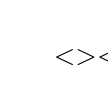
\begin{tikzpicture}
		\umlclass[x=-4, y=0]{User}
		{
			\umlstatic{userId : int} $<$PK$>$ \\
			addressId : int $<$FK$>$ \\
		}
		{
			name : varchar(255) \\
			surname : varchar(255) \\
		}

		\umlclass[x=4, y=0]{Address}
		{
			\umlstatic{addressId : int} $<$PK$>$ \\
			userId : int $<$FK$>$ \\
		}
		{
			street : varchar(255) \\
			streetNo : int \\
			flatNo : int \\
			postalCode : varchar(32) \\
			city : varchar(128) \\
			country: varchar(128) \\
		}
		\umluniassoc[mult1=1, mult2=0..1]{User}{Address}
		\node at (0.0, 0.25) {\footnotesize has};
	\end{tikzpicture}

	\caption{Modelowanie adresu użytkownika w~relacyjnej bazie danych.}
	\label{fig:er_user_address}
\end{figure}

Model ten można dokładnie odwzorować w~Apache Cassandra, jednakże jest to rozwiązanie niewydajne. Charakterystyka bazy sprawia, że sprawdzenie kraju zamieszkania użytkownika wymaga wykonania dwóch osobnych zapytań: pobrania użytkownika, a~następnie wskazywanego przez odpowiadający mu wiersz adresu. Czas przeznaczony na wykonanie jednego zapytania można aproksymować wzorem:

\begin{equation}
	t_{SELECT} = t_{AC} + t_{HASH} + t_{CN} + t_{GET} + t'_{CN} + t'_{AC}
	\label{eq:select_time}
\end{equation}

gdzie $t_{AC}$, ~$t'_{AC}$ to czas komunikacji (i~komunikacji zwrotnej) pomiędzy aplikacją a~koordynatorem, $t_{CN}$, ~$t'_{CN}$ to czas komunikacji (i~komunikacji zwrotnej) pomiędzy koordynatorem a~węzłem przechowującym wyszukiwany wiersz, $t_{HASH}$ to czas obliczania funkcji skrótu dla klucza danego wiersza, a~$t_{GET}$ to właściwy czas pobrania wiersza. Pomiędzy czynnikami zachodzi zależność:

\begin{equation}
 t_{AC}, t'_{AC}, t_{CN}, t'_{CN} >> t_{HASH}, t_{GET}.
\end{equation}

Wynika stąd, że wykonanie dodatkowego zapytania wprowadza opóźnienia związane głównie z~połączeniem pomiędzy poszczególnymi maszynami. Opóźnienia te w~większości przypadków są relatywnie niskie (rzędu kilku milisekund), więc nie jest to krytyczny problem wydajnościowy. Ponieważ można ich uniknąć, należy traktować je jako błąd projektowania modelu.

Ze względu na specyfikę modelu danych Apache Cassandry poprawnym podejściem do projektowania schematu danych jest wyjście od definicji encji i~wykonywanych na nich zapytań. Należy zauważyć, że zapytanie jest w~pewnym sensie nadzbiorem w~stosunku do relacji. Nie tylko zawiera ono informację, że dwa obiekty są ze sobą połączone, ale reprezentuje też sposób tego połączenia pozwalający na uzyskanie wymaganych informacji. Ponieważ zapytania najczęściej odwołują się do połączonych fragmentów wielu encji podstawowym ,,narzędziem'' modelowania Cassandry jest denormalizacja. Jest to zasadne zwłaszcza w~kontekście wydajnych operacji zapisu, które oferuje baza.

Niech w~przykładzie~\ref{fig:er_user_address} omawiany będzie model danych dla strony internetowej, na której występują następujące odwołania do modelu danych:

\begin{enumerate}
	\item \label{enum:username_flag} W~głównym szablonie strony przewidziane jest miejsce na nazwę użytkownika i~flagę, które są wyświetlane po zalogowaniu się.
	\item \label{enum:user_city_country} W~panelu administracyjnym wyświetlana jest lista użytkowników, która może być filtrowana po mieście i~kraju zamieszkania. Nie są na niej prezentowane pełne dane adresowe.
	\item \label{enum:full_address} Pełny adres jest widoczny po kliknięciu na osobną podstronę profilu użytkownika.
\end{enumerate}

Z~punktów \ref{enum:username_flag}~i~\ref{enum:user_city_country} wynika, że w~kontekście użytkownika pobierane są tylko dwie składowe adresu: kraj i~miasto. W~przypadku punktu~\ref{enum:full_address} można wykonać osobne zapytanie, gdyż adres wyświetlany jest na podstronie. Poprawny projekt modelu danych, który umożliwia ściąganie kompletu wymaganych danych w~jednym zapytaniu, został schematycznie przedstawiony na diagramie~\ref{tab:address_denormalization_example}.

\begin{figure}[ht!]
	\centering

	\begin{tabular}{|l||c|c|c|c|c|}
		\hhline{|-||-----|}
		 & \textbf{name} & \textbf{surname} & \textbf{addressId} & \textbf{city} & \textbf{country} \\
		\hhline{|~||=====|}
		\textbf{982} & Jakub & Turek & 1842 & Warsaw & Poland \\
		\hhline{|-||-----|}
	\end{tabular} 

	\caption{Poprawne rozwiązanie problemu modelowania użytkownika i~adresu dla zadanych wymagań.}
	\label{tab:address_denormalization_example}
\end{figure}

Silna denormalizacja pozwala na budowanie efektywnych i~bardzo szybkich modeli danych. W~zamian wymaga ona dużego nakładu planowania. Wprowadzanie zmian do modelu zdenormalizowanego jest trudne, gdyż struktura istniejących danych jest bardzo usztywniona. W~niektórych przypadkach uzysk wydajności wynikający z~wykorzystania struktury zdenormalizowanej na korzyść znormalizowanej jest niewielki, a~poniesione koszta sprawiają, że cały proces jest nieopłacalny. Z~tego względu mechanizm OMC zapewnia szerszy wybór narzędzi do modelowania zależności pomiędzy elementami modelu danych. Narzędzia te odzwierciedlają rozważania opublikowane na blogu technologicznym portalu aukcyjnego eBay - jednego z~większych użytkowników Apache Cassandry.~\cite{modeling_best_practices_pt_1}.

OMC posiada trzy wbudowane tryby, które automatyzują proces zarządzania zależnościami między danymi. Różnią się one pomiędzy sobą wydajnością (mierzoną w~liczbie zapytań niezbędnych do pobrania kompletu wymaganych danych) oraz stopniem normalizacji:

\begin{description}
	\item[Denormalizacja przez pole] Umożliwia włączenie zdenormalizowanych pól do zamodelowanej encji. Tworzy model jednostopniowy (do pobrania kompletu informacji wymagane jest jednokrotne pobranie wiersza z~tabeli).
	\item[Denormalizacja przez tabelę] Umożliwia ekstrahowanie wszystkich zdenormalizowanych zależności do osobnej tabeli. Tworzy model dwustopniowy (do pobrania kompletu informacji wymagane jest dwukrotne pobranie wiersza - z~tabeli nadrzędnej oraz tabeli zdenormalizowanej).
	\item[Normalizacja przez tabelę] Umożliwia wiązanie zależności poprzez osobną tabelę. Tworzy model trzystopniowy (do pobrania kompletu informacji wymagane jest trzykrotne pobranie wiersza - z~tabeli nadrzędnej, tabeli mapowania oraz tabeli wskazywanej).
\end{description}

\subsection{Denormalizacja przez pole}

Mechanizm denormalizacji przez pole pozwala wskazać encję, której wybrane pola zostaną automatycznie dołączone w~wybrane miejsce modelu. Po wskazaniu encji zależnej domyślnie przenoszony jest klucz partycjonowania tej encji. Jest on również dołączany do klucza klastrowania modelu. Dzięki temu możliwe jest zdefiniowanie wielu połączeń i~docieranie od obiektu nadrzędnego do obiektu zależnego. 

Denormalizacja przez pole wykorzystuje typ \verb+DenormalizedField+. Jego działanie zostanie omówione na podstawie definicji danych zawartej na diagramie~\ref{tab:address_denormalization_example}. Listing~\ref{lst:denormalization_by_field_address_entity} przedstawiono definicję encji adres zapisaną w~OCM. Model użytkownika został pokazany na listingu~\ref{lst:denormalization_by_field_example}. 

\begin{verbbox}
class Address(Model):
    address_id = UuidField(partitioning_key=True)
    street = TextField()
    street_no = IntegerField()
    flat_no = IntegerField()
    postal_code = TextField(length=32)
    city = TextField()
    country = TextField()
\end{verbbox}

\begin{figure}[ht!]
	\centering
	\theverbbox
	\caption{Denormalizacja przez pole - definicja encji adres.}
	\label{lst:denormalization_by_field_address_entity}
\end{figure}

\begin{verbbox}
class User(Model):
    user_id = UuidField(partitioning_key=True)
    name = TextField()
    surname = TextField()
    address = DenormalizedField(relates=Address, 
                                fields=['city', 'country'])
\end{verbbox}

\begin{figure}[ht!]
	\centering
	\theverbbox
	\caption{Denormalizacja przez pole - definicja encji użytkownik.}
	\label{lst:denormalization_by_field_example}
\end{figure}

Pole \verb+DenormalizedField+ używa dwóch parametrów konfiguracyjnych. Opcja \verb+relates+ przechowuje nazwę modelu, który jest wskazywany przez dane pole. Parametr \verb+fields+ definiuje nazwy pól encji wskazywanej, które mają zostać włączone do definicji modelu. Ważne jest, że w~celu uniknięcia kolizji nazw dołączane pola nazywane są według specjalnego klucza łączącego nazwę pola w~modelu nadrzędnym z~polami w~encji zależnej. W~podanym przykładzie dołączane pola będą miały nazwy: \verb+address_address_id+, \verb+address_city+ oraz \verb+address_country+.

W~porównaniu do ręcznej denormalizacji użycie pola \verb+DenormalizedField+ wprowadza liczne usprawnienia:

\begin{itemize}
	\item Cały klucz partycjonowania encji wskazywanej jest automatycznie włączany do modelu. Dzięki temu zawsze możliwe jest przejście od obiektu nadrzędnego do podrzędnego.
	\item Wykorzystanie zasady DRY\footnote{Don't Repeat Yourself (ang. ,,nie powtarzaj się'') - zasada, która w~kontekście programowania zaleca powielania tych samych lub bardzo podobnych fragmentów kodu w~wielu miejscach.} przy definiowaniu denormalizowanych pól. Gdyby w~modelu Address typ pola \verb+country+ został zmieniony na \verb+IntegerField()+ (kod kraju zamiast nazwy), typ denormalizowanego pola w~modelu \verb+User+ zostałby automatycznie uaktualniony.
	\item Generowany jest mechanizm automatycznego rozpakowywania wartości denormalizowanych z~obiektu modelu. Zakładając, że zmienna \verb+address+ przechowuje obiekt typu \verb+Address+, a~\verb+user+ obiekt typu \verb+User+, wywołanie \verb+user.address = address+ spowoduje automatyczne przypisanie wartości pól \verb+address_*+ zmiennej \verb+user+.
	\item Generowana jest metoda do automatycznego pobierania wskazywanego wiersza danych. Wywołanie \verb+user.address.get()+ zwróci obiekt typu \verb+Address+, pod warunkiem, że klucz \verb+user.address_address_id+ jest poprawny.
	\item W~przypadku aktualizacji danych encji zależnej mechanizm potrafi na życzenie zaktualizować również wszystkie zdenormalizowane wartości, które wskazują na ten obiekt. Można tego dokonać wywołując metodę \verb+update(update_related=True)+ na obiekcie modelu.
\end{itemize}

Pole \verb+DenormalizedField+ można używać również przy pustej liście parametru \verb+fields+. Wtedy dowiązywany jest wyłącznie identyfikator encji zależnej. Możliwe jest również korzystanie z~funkcji \verb+get()+, która pobierze obiekt reprezentujący zależny wiersz.

Denormalizacja przez pole jest najbardziej efektywnym czasowo sposobem modelowania relacji. Wynikowy model danych jest tożsamy z~przedstawionym na diagramie~\ref{tab:address_denormalization_example}.

\subsection{Denormalizacja przez tabelę}

Mechanizm denormalizacji przez tabelę działa analogicznie do denormalizacji przez pola, z~następującymi różnicami:

\begin{itemize}
	\item Zdenormalizowane dane przechowywane są w~osobnej tabeli, a~nie w~obiekcie nadrzędnym. 
	\item Zdenormalizowane dane nie są dostępne bezpośrednio jako pola obiektu, z~którego następuje odwołanie. 
	\item Domyślnie (przy braku specyfikacji listy pól) denormalizowane są wszystkie pola obiektu zależnego.
\end{itemize}

Na listingu~\ref{lst:denormalization_by_table_example} przedstawiono przykład denormalizacji przez tabelę opisanej jako model OMC. Ze względu na brak wyspecifikowanych pól (parametr \verb+fields+) do tabeli denormalizacyjnej zostaną włączone wszystkie pola modelu \verb+Address+. Schemat tabeli denormalizacyjnej, która powstanie na skutek zadeklarowania przykładowego modelu został zaprezentowany na diagramie~\ref{tab:address_denormalization_by_table_example}.

\begin{verbbox}
class User(Model):
    user_id = UuidField(partitioning_key=True)
    name = TextField()
    surname = TextField()
    address = DenormalizedTable(relates=Address, model='UserAddress')
\end{verbbox}

\begin{figure}[ht!]
	\centering
	\theverbbox
	\caption{Denormalizacja przez tabelę - definicja encji użytkownik.}
	\label{lst:denormalization_by_table_example}
\end{figure}

\begin{figure}[ht!]
	\centering

	\begin{tabular}{|l||c|c|c|c|c|c|}
		\hhline{|-||------|}
		 & \textbf{addressId} & \textbf{street} & \textbf{street\_no} & \textbf{postal\_code} & \textbf{city} & \textbf{country} \\
		\hhline{|~||======|}
		\textbf{233} & 754 & Nowowiejska & 15/19 & 00-665 & Warsaw & Poland \\
		\hhline{|-||------|}
	\end{tabular} 

	\caption{Denormalizacja z~wykorzystaniem tabeli. Wszystkie zdenormalizowane informacje są przechowywane w~osobnej tabeli.}
	\label{tab:address_denormalization_by_table_example}
\end{figure}

Do obsługi zdenormalizowanej tabeli generowana jest prosta klasa modelu. Opakowuje ona dostęp do zdenormalizowanych pól. Parametr \verb+model+ specyfikuje nazwę klasy tego modelu, którą następnie można wykorzystywać w~kodzie. Dostęp do wartości zdenormalizowanych dostępny jest po pobraniu obiektu zależnego. Zakładając, że zmienna \verb+user+ jest instancją klasy \verb+User+, wywołanie \verb+user.address.get()+ zwraca dane z~wiersza zdenormalizowanej tabeli. Z~wyniku wykonania metody można uzyskać później wartości pól, przykładowo \verb+user.address.get().postal_code+ dla kodu pocztowego. 

\subsection{Normalizacja przez tabelę}
\label{sec:normalization_by_table}

Normalizacja przez tabelę polega na wyekstrahowaniu mapowania identyfikatorów encji wzajemnie zależnych $(id_{relates}, id_{related})$ do osobnej tabeli. Na poziomie modelu danych przypomina to wykorzystanie tabeli pośredniczącej do modelowania relacji wiele-do-wielu w~relacyjnych bazach danych. Podstawową różnicą jest jednak brak zwrotności. Tabela normalizująca opisuje połączenie jednokierunkowe i~nie ma możliwości efektywnego odwrócenia tego związku bez utworzenia kolejnej tabeli normalizującej w~drugim kierunku.

Przykład wykorzystania normalizacji przez tabelę w~modelu OMC został przedstawiony na listingu~\ref{lst:normalization_by_table_example}. Fizyczny model danych stworzony dla przykładowego opisu przedstawia diagram~\ref{tab:address_normalization_table_data_model}. Mapowanie powiązań w~OMC przy pomocy tabeli normalizacyjnej (\verb+user_address_norm_table+) zachodzi niejawnie. Wywołanie w~kodzie aplikacji metody \verb+user.address.get()+ zwracającej listę adresów użytkownika wykonuje wiele odwołań do bazy danych. Pierwsze pobiera z~tabeli normalizującej wszystkie identyfikatory powiązanych obiektów. Kolejne zapytania ściągają do pamięci szczegóły tych obiektów.

\begin{verbbox}
class User(Model):
    user_id = UuidField(partitioning_key=True)
    name = TextField()
    surname = TextField()
    address = NormalizedTable(relates=Address)
\end{verbbox}

\begin{figure}[ht!]
	\centering
	\theverbbox
	\caption{Normalizacja przez tabelę - implementacja encji użytkownik.}
	\label{lst:normalization_by_table_example}
\end{figure}

\begin{figure}[ht!]
	\centering

	\begin{tabular}{ll}
		user\_address\_norm\_table &
		\begin{tabular}{|l||c|}
			\hhline{|-||-|}
		 	& \textbf{addressId} \\
			\hhline{|~||=|}
			\textbf{583} & 678 \\
			\hhline{|-||-|}
		\end{tabular} 	
	\end{tabular}
	
	\vspace{1em}

	\begin{tabular}{ll}
		address &
		\begin{tabular}{|l||c|c|c|c|c|}
			\hhline{|-||-----|}
		 	& \textbf{street} & \textbf{street\_no} & \textbf{postal\_code} & \textbf{city} & \textbf{country} \\
			\hhline{|~||=====|}
			\textbf{678} & Nowowiejska & 15/19 & 00-665 & Warsaw & Poland \\
			\hhline{|-||-----|}
		\end{tabular} \\
	\end{tabular}

	\caption{Model danych tabeli normalizacyjnej. Identyfikatorem wiersza w~tabeli \emph{user\_address\_norm\_table} jest identyfikator użytkownika.}
	\label{tab:address_normalization_table_data_model}
\end{figure}

Na podstawie opisu działania metody \verb+get()+ łatwo stwierdzić, że takie rozwiązanie bardzo źle skaluje się ze wzrostem gęstości połączeń. Przeciętna ilość zapytań niezbędnych do pobrania kompletu informacji z~bazy danych wynosi:

\begin{equation}
|q_{avg}| = 1 + r_{avg}
\end{equation}

gdzie $r_{avg}$ jest średnią liczbą obiektów wskazywanych przez encję nadrzędną. Dla licznych, gęstych zbiorów danych oznacza to występowanie sytuacji, w~których należy $n$ osobnych zapytań dla wszystkich $n$ elementów zapytań, które znajdują się w~zbiorze.

\subsection{Porównanie wydajności metod zarządzania zależnościami}

Trzy zaprezentowane metody różnią się od siebie wydajnością poszczególnych operacji w~kontekście charakterystyki danych. Aby ułatwić wybór rodzaju modelowania w~zależności od scenariusza użytkownia Autor przeprowadził szereg testów wydajnościowych, które ukazują zalety i~wady poszczególnych typów modelowania. Wszystkie testy zostały przeprowadzone dla modelu danych użytkowników i~przypisanych do nich adresów.

\paragraph{Skalowalność operacji wyszukiwania względem gęstości połączeń} 

Celem pierwszego testu jest zbadanie zależności pomiędzy wydajnością operacji pobierania kompletu danych, a~gęstością połączeń pomiędzy encjami zależnymi. Gęstość połączeń to średnia ilość podzależnych elementów przypadających na jeden element nadrzędny. 

W~trakcie testu zostało wygenerowanych 10000 użytkowników oraz 1000 adresów. W~poszczególnych iteracjach mierzone były czas pobierania wszystkich użytkowników, wraz ze wszystkimi wymaganymi informacjami adresowymi, ale dla różnej gęstości połączeń pomiędzy danymi. Wyniki testu zostały przedstawione na wykresie~\ref{fig:select_time_relation_density_comparison}.

\begin{figure}[ht!]
	\centering
	\begin{tikzpicture}
		\begin{axis}[
				width=.8\textwidth,
				xlabel=Czas wyszukiwania kompletu informacji ($s$),
				ylabel=Średnia gęstość zależności,
				scaled ticks=false, 
				tick label style={/pgf/number format/fixed},
				legend style={at={(0.95,0.15)},anchor=east}
			]
			\addplot[color=red] coordinates {
				(65.050, 100)
				(58.103, 75)
				(49.212, 50)
				(40.119, 25)
				(33.882, 10)
			};
			\addlegendentry{Denormalizacja przez pola}

			\addplot[color=green] coordinates {
				(120.885, 100)
				(106.164, 75)
				(99.982, 50)
				(80.021, 25)
				(66.424, 10)
			};
			\addlegendentry{Denormalizacja przez tabelę}

			\addplot[color=blue] coordinates {
				(1587.503, 100)
				(1314.820, 75)
				(946.212, 50)
				(591.928, 25)
				(227.424, 10)
			};
			\addlegendentry{Normalizacja przez tabelę}
		\end{axis}
	\end{tikzpicture}

	\caption{Porównanie czasu pobierania informacji dla różnych metod modelowania zależności (przy rosnącej gęstości połączeń).}
	\label{fig:select_time_relation_density_comparison}
\end{figure}

Z~wykresu można odczytać ogromną przewagę modeli zdenormalizowanych nad modelem znormalizowanym przy masowym odczycie wielu rekordów. Jest to zgodne z~prognozami przedstawionymi w~sekcji~\ref{sec:normalization_by_table}. Liczba zapytań potrzebnych do pobrania kompletu informacji z~wykorzystaniem normalizacji przez tabelę rośnie wraz ze wzrostem encji w~zbiorze danych, jak również z~gęstością połączeń. Uzyskany wykres ma charakterystykę nieliniową. W~przypadku denormalizacji przez pola/tabelę uzyskane wyniki mają charakterystykę w~przybliżeniu liniową. Ilość wykonywanych zapytań zależy wyłącznie od liczby elementów w~zbiorze danych.

Należy zauważyć, że wykres nie oddaje pełni różnic pomiędzy modelami. Ponieważ czas dostępu dla zależności znormalizowanej odbiega znacząco od pozostałych, skala nie odzwierciedla różnicy pomiędzy podejściami zdenormalizowanymi. Zgodnie z~przewidywaniami mechanizm denormalizacji przez pole jest dla wszystkich punktów pomiaru w~przybliżeniu dwukrotnie szybszy od denormalizacji przez tabelę, ponieważ do pobrania informacji należy wykonać dwa razy mniej zapytań.

\paragraph{Skalowalność operacji wyszukiwania względem ilości encji}

Celem tego testu jest zbadanie szybkości wyszukiwania kompletu danych, kiedy gęstość połączeń w~modelu jest stała, a~zmienia się ilość encji nadrzędnych oraz zależnych. Wszystkie badania zostały przeprowadzone dla średniej gęstości połączeń wynoszącej 10. W~kolejnych iteracjach liniowo zwiększana była ilość wierszy użytkownika i~ilość adresów. Wyniki badań zostały przedstawione na wykresie~\ref{fig:select_time_relation_quantity_comparison}.

\begin{figure}[ht!]
	\centering
	\begin{tikzpicture}
		\begin{axis}[
				width=.8\textwidth,
				xlabel=Czas wyszukiwania kompletu informacji ($s$),
				ylabel=Ilość użytkowników/adresów,
				scaled ticks=false, 
				tick label style={/pgf/number format/fixed},
				ytick={5000, 10000, 20000, 40000},				
				yticklabels={5000 / 500, 10000 / 1000, 20000 / 2000, 40000 / 4000},
				yticklabel style={text width=2.5cm, align=right, /pgf/number format/fixed},
				legend style={at={(0.95,0.15)},anchor=east}
			]
			\addplot[color=red] coordinates {
				(154.221, 40000)
				(72.077, 20000)
				(33.882, 10000)
				(15.623, 5000)
			};
			\addlegendentry{Denormalizacja przez pola}

			\addplot[color=green] coordinates {
				(279.663, 40000)
				(137.108, 20000)
				(66.424, 10000)
				(31.974, 5000)
			};
			\addlegendentry{Denormalizacja przez tabelę}

			\addplot[color=blue] coordinates {
				(947.889, 40000)
				(468.024, 20000)
				(227.424, 10000)
				(113.211, 5000)
			};
			\addlegendentry{Normalizacja przez tabelę}
		\end{axis}
	\end{tikzpicture}

	\caption{Porównanie czasu pobierania informacji dla różnych metod modelowania zależności (przy rosnącej ilości wierszy).}
	\label{fig:select_time_relation_quantity_comparison}
\end{figure}

Kolejny raz efektywność zależności znormalizowanej przez tabelę znacząco odstaje od efektywności zależności zdenormalizowanych. Jednakże w~przeciwieństwie do gęstości zależności, zwiększanie liczby wierszy powoduje liniowy wzrost czasu potrzebnego na pobranie kompletu danych. Wynika z~tego, że model zdenormalizowany dużo lepiej sprawdza się w~przypadku rzadkich zbiorów połączeń pomiędzy encjami. Podobnie jak w~przypadku poprzedniego badania, model zdenormalizowany poprzez pola okazuje się dwa razy szybszy od denormalizacji z~użyciem osobnej tabeli.

\paragraph{Skalowalność operacji aktualizacji względem gęstości połączeń} 

Celem testu jest porównanie szybkości aktualizacji danych zależnych w~przypadku różnych typów modelowania. W~trakcie testu zostało wygenerowanych 10000 użytkowników i~1000 adresów. Zmieniana była gęstość połączeń pomiędzy encjami danych. Aktualizacji podlegały wszystkie elementy ze zbioru zależnych danych (adresy). Wyniki testu zostały przedstawione na wykresie~\ref{fig:update_time_relation_density_comparison}.

\begin{figure}[ht!]
	\centering
	\begin{tikzpicture}
		\begin{axis}[
				width=.8\textwidth,
				xlabel=Czas aktualizacji kompletu informacji ($s$),
				ylabel=Średnia gęstość zależności,
				scaled ticks=false, 
				tick label style={/pgf/number format/fixed},
				legend style={at={(0.95,0.15)},anchor=east},
				xtick = {0, 300, 600, 900, 1200, 1500, 1800, 2100}
			]
			\addplot[color=red] coordinates {
				(2137.998, 100)
				(1098.212, 50)
				(547.172, 25)
				(164.962, 10)
			};
			\addlegendentry{Denormalizacja}

			\addplot[color=green] coordinates {
				(26.434, 100)
				(25.981, 50)
				(26.423, 25)
				(26.719, 10)
			};
			\addlegendentry{Normalizacja przez tabelę}
		\end{axis}
	\end{tikzpicture}

	\caption{Porównanie czasu aktualizacji informacji dla różnych metod modelowania zależności (przy rosnącej gęstości połączeń).}
	\label{fig:update_time_relation_density_comparison}
\end{figure}

Z~wykresu wynika, że czas aktualizacji rekordów znormalizowanych jest niezależny od gęstości połączeń. W~modelu znormalizowanym wystarczy zaktualizować wszystkie encje zależne, więc mierzony czas faktycznie powinien być stały względem gęstości. Aktualizacja modelu znormalizowanego jest bardzo efektywna. Czas aktualizacji 1000 przedmiotów na środowisku lokalnym (przetwarzanie jednowątkowe) wynosił niewiele poniżej 30 sekund. 

Oba modele zdenormalizowane mają fatalną wydajność aktualizacji kompletu danych. Problemem jest brak możliwości efektywnego wyszukiwania identyfikatorów wszystkich użytkowników, którzy są powiązani z~danym adresem. Klauzula aktualizacji w~Apache Cassandra nie wspiera wykorzystania indeksów drugiego stopnia. Bez wykorzystania indeksów drugiego stopnia nie jest możliwe znalezienie encji nadrzędnych, które są powiązane z~daną encją zależną. Stąd wykonanie zestawu operacji \verb+UPDATE+ jest zawsze poprzedzone wyszukiwaniem \verb+SELECT+. Kolejną przeszkodą jest ilość aktualizowanych danych. W~przypadku modelu znormalizowanego wystarczyło wykonanie $|Z|$ operacji, gdzie $Z$~to zbiór elementów zależnych (adresów). Dla modelu zdenormalizowanego liczba ta jest zwielokrotniona przez średnią gęstość połączeń pomiędzy wierszami.

\paragraph{Skalowalność operacji aktualizacji względem ilości encji}

Celem testu jest porównanie szybkości aktualizacji danych zależnych w~przypadku stałej gęstości zależności dla różnych typów modelowania. Średnia gęstość w~trakcie wszystkich iteracji testów wynosi 10. Liniowo zmieniają się natomiast liczby wierszy w~tabelach użytkowników i~adresów. Wyniki testu zostały przedstawione na wykresie~\ref{fig:update_time_relation_quantity_comparison}.

\begin{figure}[ht!]
	\centering
	\begin{tikzpicture}
		\begin{axis}[
				width=.8\textwidth,
				xlabel=Czas aktualizowania kompletu informacji ($s$),
				ylabel=Liczba wierszy użytkowników / adresów,
				scaled ticks=false, 
				ytick={5000, 10000, 20000, 40000},				
				yticklabels={5000 / 500, 10000 / 1000, 20000 / 2000, 40000 / 4000},
				yticklabel style={text width=2.5cm, align=right, /pgf/number format/fixed},
				tick label style={/pgf/number format/fixed},
				legend style={at={(0.95,0.15)},anchor=east}
			]
			\addplot[color=red] coordinates {
				(457.816, 40000)
				(262.216, 20000)
				(164.962, 10000)
				(97.575, 5000)
			};
			\addlegendentry{Denormalizacja}

			\addplot[color=green] coordinates {
				(109.982, 40000)
				(54.231, 20000)
				(26.719, 10000)
				(13.123, 5000)
			};
			\addlegendentry{Normalizacja przez tabelę}
		\end{axis}
	\end{tikzpicture}

	\caption{Porównanie czasu aktualizacji informacji dla różnych metod modelowania zależności (przy rosnącej ilości wierszy).}
	\label{fig:update_time_relation_quantity_comparison}
\end{figure}

Podobnie jak w~poprzednim badaniu wydajności aktualizacji, efektywniejszy okazał się model znormalizowany. Mierzony czas rośnie proporcjonalnie do ilości nadpisywanych rekordów. Dla zadanego problemu jest to rozwiązanie optymalne.

W~przypadku denormalizacji można zauważyć, że wzrost liczby wierszy w~tabeli ma łagodniejszy wpływ na charakterystykę wykresu czasu aktualizacji niż rosnąca gęstość połączeń. Przykładowo dwukrotny wzrost gęstości połączeń odnosi podobny skutek czasowy co ośmiokrotny wzrost ilości danych. 

\subsection{Wnioski z~analizy wydajności modelowania zależności}

Nie ma uniwersalnego sposobu, który pozwala na uzyskanie optymalnego wyniku przy mapowaniu zależności w~Apache Cassandra. Dobór metody powinien zależeć od charakterystyki przechowywanych danych. 

Szukając pewnego rodzaju uogólnienia Autor wprowadził pomocniczą definicję typowego zbioru danych. Posiada on zbiór następujących cech:

\begin{itemize}
	\item Duża liczba wierszy w~zbiorze ($> 100000$).
	\item Operacje wyszukiwania są znacznie częstsze niż aktualizacji. Stosunek częstotliwości ich występowania wynosi $20 \div 1$ (istnieje $5\%$ szansy, że użytkownik przeglądający profil zaktualizuje dane adresowe).
	\item Gęstość występowania zależności jest niewielka. Na jeden wiersz encji nadrzędnej przypada średnio nie więcej niż dziesięć wierszy encji zależnej. 
\end{itemize}

Dla tak określonego zbioru danych zdecydowanie najlepszym wyborem jest modelowanie z~wykorzystaniem denormalizacji poprzez pola. Głównym kryterium jest tutaj znacząca przewaga w~czasie wyszukiwania danych i~akceptowalny narzut przeznaczony na aktualizację danych. Liczne artykuły prezentujące studium przypadku użycia Apache Cassandry każą sądzić, że ten rodzaj modelowania zależności jest prawdopodobnie najlepiej dostosowany do specyfiki schematu danych. 

W~przypadku małych zbiorów danych (preferowana ilość wierszy w~tabelach $\leq 10000$) o~niskiej gęstości zależności warto rozważyć użycie reprezentacji znormalizowanej. Nie jest ona obarczona narzutem na aktualizację danych. Zaletą tej reprezentacji jest większa elastyczność schematu. W~przeciwieństwie do postaci zdenormalizowanej, gdzie może zdarzyć się, że przy dodaniu kolejnego zapytania trzeba rozszerzyć tabelę denormalizacji o~kolejną kolumnę, zapewnia on dostęp do kompletu danych bez konieczności wprowadzania zmian w~strukturze. 

Reprezentacja zdenormalizowana jest zalecana w~przypadku, gdy wyszukiwanie danych nie jest kluczowym kryterium. Przykładem mogą być dane służące do generacji raportów, gdzie liczba aktualizacji może znacznie przewyższać liczbę wyszukiwań. 

Duży problem stanowi modelowanie zależności o~dużej liczbie połączeń między danymi. Wraz ze wzrostem gęstości połączeń możliwości zawężają się do:

\begin{itemize}
	\item Zaniedbania aktualizacji zdenormalizowanych danych. W~praktyce jest to bardzo kłopotliwe i~może być zastosowane jeżeli udaje się zdenormalizowanie wyłącznie danych przeznaczonych tylko do odczytu.
	\item Poświęcenia czasu aktualizacji kosztem czasu dostępu do danych i~wyboru modelu zdenormalizowanego.
	\item Poświęcenia czas dostępu do danych kosztem czasu aktualizacji i~wyboru modelu znormalizowanego.
	\item Zmiany modelowania danych w~taki sposób, aby zredukować zagęszczenie zależności.
\end{itemize}

Jeżeli żadna z~powyższych możliwości nie daje się zastosować lub nie wprowadza akceptowalnej poprawy wydajności należy rozważyć wybór innego silnika bazodanowego. Dla zbiorów o~bardzo gęstej siatce zależności naturalne zastosowanie mają grafowe bazy danych. Przykładem dojrzałego projektu silnika grafowego o~dobrych własnościach skalowania jest Neo4j\footnote{Strona domowa projektu Neo4j dostępna jest pod adresem \url{http://www.neo4j.org}.}. 

\begin{figure}[ht!]
	\centering
	\begin{tikzpicture}
		\begin{axis}[
				width=.8\textwidth,
				xlabel=Czas aktualizacji kompletu informacji ($s$),
				ylabel=Średnia gęstość zależności,
				scaled ticks=false, 
				tick label style={/pgf/number format/fixed},
				legend style={at={(0.95,0.15)},anchor=east},
				xtick = {0, 300, 600, 900, 1200, 1500, 1800, 2100}
			]
			\addplot[color=red] coordinates {
				(2137.998, 100)
				(1098.212, 50)
				(547.172, 25)
				(164.962, 10)
			};
			\addlegendentry{Aktualizacja}

			\addplot[color=green] coordinates {
				(1165.276, 100)
				(640.261, 50)
				(355.701, 25)
				(162.771, 10)
			};
			\addlegendentry{Wstawianie}
		\end{axis}
	\end{tikzpicture}

	\caption{Porównanie czasu wstawiania i~aktualizacji informacji (przy rosnącej gęstości połączeń).}
	\label{fig:update_vs_insert_time_density_comparison}
\end{figure}

\section{Wsparcie dla wzorców modelowania}

Jednym z~pryncypiów projektowych mechanizmu OMC jest obsługa wzorców modelowania. W~literaturze zostały zebrane i~opisane liczne przykłady efektywnych i~nieefektywnych projektów modelu danych dla Apache Cassandry. Z~przeanalizowanych opisów Autor wybrał zbiór reużywalnych wzorców. Następnie, dla każdego wzorca, przygotowany został mechanizm, który ułatwia jego modelowanie w~środowisku OMC. Dzięki temu mechanizm został wzbogacony o~obsługę:

\begin{itemize}
	\item Szeregów zdarzeń, czyli zbioru uporządkowanych względem czasu wiadomości.
	\item Kolejek \emph{First In, First Out}, \emph{Last In, Last Out} i~podobnych.
	\item Indeksów wartości unikalnych. 
	\item Aktualizacji selektywnej.
\end{itemize}

\subsection{Szereg zdarzeń}

Apache Cassandra została zaprojektowana z~myślą o~wspieraniu szeregów zdarzeń. Szereg zdarzeń to uporządkowane względem czasu wystąpienia wpisy do bazy danych, które opcjonalnie mogą posiadać z~góry określony czas życia. Typowym przykładem szeregu zdarzeń są wartości odczytów z~urządzeń pomiarowych. Wartości te zwyczajowo są pobierane cyklicznie, a~do wykorzystania w~czasie rzeczywistym przydatne są tylko najnowsze odczyty. Doskonały opis modelowania szeregów zdarzeń przedstawiony jest we wpisie Patricka McFadina na portalu \textbf{Planet Cassandra}.~\cite{time_series_modeling_pattern} Artykuł analizuje przykład stacji meteorologicznych. Przedstawia trzy sposoby zapisu szeregu zdarzeń w~Apache Cassandra. 

\paragraph{Odczyty dla tego samego urządzenia w~pojedynczym wierszu} 

Najprostszą możliwością jest zebranie wszystkich próbek dla danego urządzenia w~jednym wierszu tabeli. Kolejne wartości zapisywane są ze śladem czasu w~nazwie kolumny. Listing~\ref{lst:time_series_modeling_one} przedstawia wzorzec zapisany jako model OMC.

\begin{verbbox}
class TimeSeriesPatternOne(Model):
    weatherstation_id = TextField(partitioning_key=True)
    event_time = TimestampField(clustering_key=True, auto_on_create=True)
    temperature = TextField()
\end{verbbox}

\begin{figure}[ht!]
	\centering
	\theverbbox
	\caption{Modelowanie szeregu zdarzeń. Zapis kolejnych odczytów jako kolumny.}
	\label{lst:time_series_modeling_one}
\end{figure}

Zapis śladu czasu w~nazwie kolumny można uzyskać poprzez dołączenie pola do złożonego klucza głównego tabeli jako \emph{clustering key}\footnote{Clustering key (ang. dosłownie ,,klucz klastrowania'') - część złożonego klucza głównego tabeli, która określa w~jakiej kolejności grupowane są wpisy względem klucza partycjonowania (identyfikatora wiersza).}. Dołączenie to dokonuje się poprzez ustawienie flagi \verb+clustering_key+ na \verb+True+. 

Udogodnieniem dla programisty korzystającego z~OMC jest możliwość automatycznej generacji śladu czasu dla chwili obecnej. Ślad czasu może być wygenerowany w~trakcie tworzenia obiektu (\verb+auto_on_create=True+) lub w~trakcie wstawiania obiektu do bazy danych (\verb+auto_on_save=True+).  

\paragraph{Grupowanie odczytów dla urządzenia i~fragmentu daty} 

W~przypadku gdy odczytów jest zbyt dużo by mieściły się w~jednym wierszu sugerowanym rozwiązaniem jest dodatkowe partycjonowanie wierszy po komponencie daty: miesiącu, dniu, itd. Autor wzorca sugeruje utworzenie w~modelu dodatkowego pola, do którego wpisywany jest komponent daty i~dołączenie tego pola do klucza partycjonowania. Takie modelowanie dziedziny może prowadzić do potencjalnych błędów. Ta sama dana - ślad czasu - przechowywana jest w~dwóch polach, które różnią się formatowaniem. 

OMC posiada mechanizm partycjonowania dat po komponencie. W~modelu znajduje się tylko jedna dana - faktyczny ślad czasu. OMC na jej podstawie automatycznie tworzy i~formatuje klucz partycjonowania. Dzięki temu programista nie musi dbać o~ręczne wyznaczanie komponentu daty. Listing~\ref{lst:time_series_modeling_two} przedstawia opis modelu z~partycjonowaniem względem dnia.

\begin{verbbox}
class TimeSeriesPatternTwo(Model):
    weatherstation_id = TextField(partitioning_key=True)
    event_time = TimestampField(clustering_key=True, 
                                auto_on_create=True, 
                                partitioning_by_day=True)
\end{verbbox}

\begin{figure}[ht!]
	\centering
	\theverbbox
	\caption{Modelowanie szeregu zdarzeń. Partycjonowanie zdarzeń po komponencie daty.}
	\label{lst:time_series_modeling_two}
\end{figure}

Pole \verb+event_time+ modelu \verb+TimeSeriesPatternTwo+ jest kluczem klastrowania. Dodatkowo posiada ono ustawioną flagę \verb+partitioning_by_day=True+, która spełnia trzy zadania:

\begin{itemize}
	\item Przy tworzeniu schematu tabeli dodaje dodatkową kolumnę \verb+event_time_day+\footnote{Nazwa jest tworzona z~nazwy pola oraz nazwy komponentu daty.} o~typie tekstowym. Pole to jest automatycznie włączane do klucza partycjonowania.
	\item Przy zapisywaniu obiektu do bazy danych automatycznie wypełnia wartość dodatkowego pola o~ślad czasu obcięty do z~dokładnością do dnia.
	\item Przy wyszukiwaniu obiektów po dacie automatycznie filtruje dane zarówno po wartości pola \verb+event_time_day+, jak i~\verb+event_time+.
\end{itemize}

Dostępne jest kilka rodzajów komponentów daty, po których można dokonać partycjonowania. Różnią się one ostatnim członem nazwy parametru. Wybór obejmuje partycjonowanie po latach (\verb+_year+), miesiącach (\verb+_month+), dniach (\verb+_day+), godzinach (\verb+_hour+), minutach (\verb+_minute+) oraz sekundach (\verb+_second+).

\paragraph{Odczyty z~ograniczoną pamięcią}

Korzystając z~wbudowanego mechanizmu Cassandry możliwe jest tworzenie automatycznie przedawniających się wartości. Wstawiając pozycję do bazy danych można ustawić czas życia, po którym zostanie ona usunięta. Przedawnianie się wartości może być wykorzystywane w~połączeniu z~odwrotną kolejnością sortowania wpisów (od najnowszego do najstarszego). Dzięki temu bardzo łatwo jest budować widoki, które prezentują kilka najnowszych informacji.

OMC zapewnia dwa rodzaje wsparcia dla czasu życia wartości. Czas życia może być ustawiany dla indywidualnych obiektów. Przy zapisywaniu obiektu należy na jego instancji wywołać metodę \verb+save(ttl=20)+. Parametr \verb+ttl+ definiuje czas życia wartości w~sekundach. Czas życia można również ustawić globalnie dla wszystkich instancji modelu. Wykorzystuje się do tego pole \verb+__ttl__+ klasy. Zaprezentowano to na listingu~\ref{lst:time_series_modeling_three}.

\begin{verbbox}
class TimeSeriesPatternThree(Model):
    __ttl__ = 20
    weatherstation_id = TextField(partitioning_key=True)
    event_time = TimestampField(clustering_key=True, 
                                descending_clustering=True
                                auto_on_create=True)
    temperature = TextField()
\end{verbbox}

\begin{figure}[ht!]
	\centering
	\theverbbox
	\caption{Modelowanie szeregu zdarzeń. Przedawniające się odczyty jako kolumny z~sortowaniem od najnowszego.}
	\label{lst:time_series_modeling_three}
\end{figure} 

Dla każdego pola, które jest częścią klucza klastrowania można ustawić odwrotną kolejność sortowania elementów. Do tego celu należy ustawić flagę \verb+descending_clustering+ na \verb+True+.

\subsection{Wsparcie dla kolejek}

W~sekcji~\ref{sec:patterns_and_antipatterns} został przytoczony antywzorzec kolejki. Problem został opisany przez Alekseya Yeschenko na blogu firmy DataStax.~\cite{cassandra_queue_antipattern} Wynika on ze sposobu obsługi operacji usuwania przez silnik Apache Cassandra. Usuwanie nie jest realizowane natychmiast. Zamiast tego kasowana kolumna oznaczana jest specjalnym znacznikiem \emph{tombstone} i~rezyduje w~pamięci aż do momentu, gdy nastąpi właściwe wyrzucanie. Przy dużej liczbie usunięć kolumn z~wiersza może zdarzyć się, że zapytanie filtrujące z~limitem będzie działało znacznie wolniej niż dla wiersza z~identyczną ilością kolumn, ale bez poprzedzających usunięć. Wynika to z~faktu, że stwierdzenie, że dana wartość jest ,,martwa'' wymaga pobrania kolumny i~zdeserializowania jej wartości. Jeżeli po deserializacji wykryty zostanie znacznik \emph{tombstone}, wtedy pobierana jest kolejna wartość. Proces powtarzany jest aż do skutku.

Kolejka może być zamodelowana efektywniej w~przypadku, gdy możliwe jest wskazanie miejsca, w~którym rozpoczynają się nieusunięte kolumny. Przykładem może być kolejka typu FIFO\footnote{FIFO (First In, First Out) - rodzaj kolejki, w~którym elementy obsługiwane są według kolejności wstawienia.}. Wyszukując kolejny element w~kolejce można nałożyć warunek, że czas wstawienia elementu do kolejki jest późniejszy niż czas ostatnio usuniętego elementu. OMC dostarcza wsparcia dla takich kolejek, co zostało przedstawione na listingu~\ref{lst:fifo_queue_modeling}.

\begin{verbbox}
class FIFOQueue(Model):
    __track_deletes__ = ('enqueued_at', 'ASC')
    name = TextField(partitioning_key=True)
    enqueued_at = UuidField(type=TimeUuid, 
                            auto_generate=True, 
                            clustering_key=True)
    payload = DataField()

# create three queue elements

first_element = FIFOQueue(name = '1', payload = 'firstPayload')
second_element = FIFOQueue(name = '2', payload = 'secondPayload')
third_element = FIFOQueue(name = '3', payload = 'thirdPayload')

# save elements into database

first_element.save()
second_element.save()
third_element.save()

# delete first two elements from database

first_element.delete()
second_element.delete()

# get element with name '3'

FIFOQueue.objects().find(name='3')[:1]
\end{verbbox}

\begin{figure}[ht!]
	\centering
	\theverbbox
	\caption{Modelowanie kolejki typu FIFO w~OMC.}
	\label{lst:fifo_queue_modeling}
\end{figure}

Parametr \verb+__track_deletes__+ umożliwia śledzenie operacji usuwania. Przyjmuje on parę łańcuchów znaków: nazwę pola, którego wartość jest śledzona podczas usuwania oraz warunek zapisywania śledzonej wartości. Na chwilę obecną obsługiwane jest śledzenie pól typu \verb+UuidField+ oraz \verb+TimestampField+, a~także dwa warunki śledzenia: \verb+ASC+ oraz \verb+DESC+. Warunek \emph{ascending} oznacza, że śledzona wartość jest aktualizowana tylko w~przypadku, gdy jest mniejsza od usuwanej obecnie wartości. Warunek \emph{descending} działa odwrotnie - aktualizuje śledzoną wartość tylko w~przypadku, gdy jest większa od usuwanej obecnie.

Ustawienie parametru \verb+__track_deletes__+ powoduje, że śledzona wartość jest automatycznie dodawana do wszystkich zapytań wyszukujących obiekty. Oznacza to, że ostatnie wywołanie w~listingu~\ref{lst:fifo_queue_modeling} będzie miało ustawione trzy warunki filtrowania:

\begin{itemize}
	\item Nazwa elementu (\verb+name+) jest równa \verb+'3'+ - wynika z~\verb+find(name='3')+.
	\item Wybierz maksymalnie jeden element (\verb+LIMIT 1+) - wynika z~zakresu \verb+[:1]+.
	\item Czas dodania do kolejki (\verb+enqueued_at+) większy od \verb+second_element.enqueued_at+ - automatycznie dodawane przez OMC.
\end{itemize}

Wykorzystanie opcji \verb+__track_deletes__+ w~sposób znaczący wpływa na wydajność kolejki FIFO. Na wykresie~\ref{fig:fifo_select_time_comparison} przedstawiono porównanie szybkości działania wyszukiwania pierwszego nieusuniętego elementu kolejki przy włączonym oraz wyłączonym śledzeniu. Pomiar wydajności został przeprowadzony na lokalnej konfiguracji klastra Apache Cassandra. Czas mierzony był przez aplikację wykorzystującą mechanizm OMC. Aplikacja ta wstawiała do kolejki $y$ przedmiotów, po czym usuwała pierwsze $y-1$ przedmiotów z~tej kolejki. Mierzony był czas wyszukiwania pierwszego elementu należącego do kolejki (z~ograniczeniem \verb+LIMIT 1+, podobnie jak przy wywołaniu metody \verb+find+ w~listingu~\ref{lst:fifo_queue_modeling}). 

\begin{figure}
	\centering
	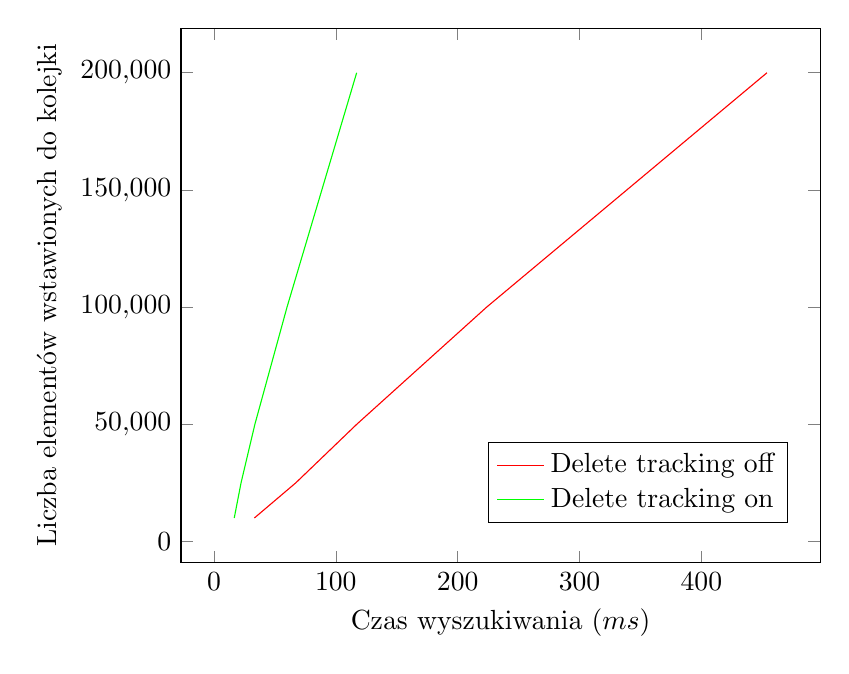
\begin{tikzpicture}
		\begin{axis}[
				width=.8\textwidth,
				xlabel=Czas wyszukiwania ($ms$),
				ylabel=Liczba elementów wstawionych do kolejki,
				scaled ticks=false, 
				tick label style={/pgf/number format/fixed},
				legend style={at={(0.95,0.15)},anchor=east}
			]
			\addplot[color=red] coordinates {
				(453.832, 200000)
				(223.832, 100000)
				(117.231, 50000)
				(67.193, 25000)
				(33.204, 10000)
			};
			\addlegendentry{Delete tracking off}

			\addplot[color=green] coordinates {
				(117.112, 200000)
				(59.973, 100000)
				(33.598, 50000)
				(22.231, 25000)
				(16.655, 10000)
			};
			\addlegendentry{Delete tracking on}
		\end{axis}
	\end{tikzpicture}

	\caption{Porównanie czasu wstawiania wielu rekordów.}
	\label{fig:fifo_select_time_comparison}
\end{figure}

Pomimo znaczącej poprawy czasu dostępu do danych przy wykorzystaniu parametru \verb+__track_deletes__+ można zauważyć, że modelowanie nie jest optymalne. W~przypadku braku usunięć danych z~tabeli czas dostępu do pojedynczej danej powinien być w~przybliżeniu stały. Z~wykresu wynika jednak, że wyszukiwanie wydłuża się wraz ze wzrostem liczby elementów w~kolejce. Pozwala to wyciągnąć wniosek, że efektywne modelowanie w~Cassandrze powinno całkowicie eliminować lub radykalnie ograniczać ilość wykonywanych operacji usunięć.

\subsection{Selektywna aktualizacja}

Apache Cassandra jest przystosowana do obsługi wielu równoległych źródeł danych. Ze względu na brak transakcyjności jednym ze sposobów na uniknięcie problemów synchronizacji jest zalecana przez Dave'a Gardnera selektywna aktualizacja.~\cite{cassandra_concepts_patterns_antipatterns} Edytując zawartość danego wiersza należy przesyłać do bazy danych wyłącznie wartości, które rzeczywiście uległy modyfikacji. Inaczej istnieje prawdopodobieństwo niecelowego nadpisania zmian wprowadzonych równolegle przez inne źródło danych. OMC domyślnie korzysta z~mechanizmu selektywnej aktualizacji, co przedstawiono na listingu~\ref{lst:selective_update_modeling}.

\begin{verbbox}
class SelectiveUpdate(Model):
    name = TextField(partitioning_key=True)
    description = TextField(length=1024)
    priority = IntegerField()

# find object with name 'su_test'
su_test = SelectiveUpdate.objects().find(name='su_test').get()

# update priority
su_test.priority = 1

# update object
su_test.save()
\end{verbbox}

\begin{figure}[ht!]
	\centering
	\theverbbox
	\caption{Przykład selektywnej aktualizacji.}
	\label{lst:selective_update_modeling}
\end{figure}

W~pierwszej kolejności metoda \verb+save()+ sprawdza, którą z~dwóch operacji, aktualizacji czy wstawienia obiektu, należy wykonać. Przy wykonywaniu aktualizacji do bazy danych przesyłana jest tylko wartość zmienionych pól, w~danym przykładzie tylko priorytetu. Jeżeli pomiędzy pobraniem obiektu, a~aktualizacją priorytetu i~zapisaniem obiektu w~bazie danych inny węzeł dokona zmiany opisu obiektu, opis ten nie zostanie ponownie nadpisany poprzednią wartością.

Mechanizm aktualizacji selektywnej można wyłączyć. Można dokonać tego wywołując metodę \verb+save()+ z~parametrem \verb+selective_update=False+. Alternatywnie selektywna aktualizacja może zostać wyłączona dla całego modelu poprzez zadeklarowanie pola \verb+__selective_update__ = False+.

\subsection{Indeks wartości unikalnych}

Aby umożliwić wyszukiwanie po wartościach kolumny, która nie należy do klucza głównego tabeli należy użyć indeksu drugiego rzędu (\emph{secondary index}). Według dokumentacji Apache Cassandry~\cite{cassandra_indexes} indeksy drugiego stopnia powinny być używane na kolumnach, które silnie grupują wiersze encji nadrzędnej. Wynika to z~wewnętrznej implementacji indeksów drugiego stopnia. Załóżmy, że w~systemie istnieje tabela przechowująca dane użytkowników, w~której zapisane są wiersze zaprezentowane na diagramie~\ref{tab:secondary_index_example_users_table}.

\begin{figure}[ht!]
	\centering

	\begin{tabular}{|l||c|c|c|c|}
		\hhline{|-||----|}
		 & \textbf{name} & \textbf{surname} & \textbf{email} & \textbf{city} \\
		\hhline{|~||====|}
		\textbf{jturek} & Jakub & Turek & J.Turek@stud.elka.pw.edu.pl & Warsaw \\
		\hhline{|=::====}
		 & \textbf{name} & \textbf{surname} & \textbf{email} & \textbf{city} \\
		\hhline{|~||====|}
		\textbf{manisero} & Michał & Aniserowicz & M.Aniserowicz@stud.elka.pw.edu.pl & Warsaw \\
		\hhline{|-||----|}
	\end{tabular} 

	\caption{Przykładowe wartości w~tabeli użytkownicy.}
	\label{tab:secondary_index_example_users_table}
\end{figure}

Przykładowy wygląd danych w~tabeli, która realizuje indeks drugiego stopnia dla miasta (kolumna \verb+city+), został zaprezentowany na diagramie~\ref{tab:secondary_index_example_index_table}.

\begin{figure}[ht!]
	\centering

	\begin{tabular}{|l||c|c|}
		\hhline{|-||--|}
		 & \textbf{jturek} & \textbf{manisero} \\
		\hhline{|~||==|}
		\textbf{Warsaw} & null & null \\
		\hhline{|-||--|}
	\end{tabular} 

	\caption{Przykładowa tabela, która mogłaby realizować indeks drugiego stopnia dla kolumny \emph{city} z~diagramu~\ref{tab:secondary_index_example_users_table}.}
	\label{tab:secondary_index_example_index_table}
\end{figure}

Wadą rozwiązania przedstawionego na diagramie~\ref{tab:secondary_index_example_index_table} jest brak skalowalności. Przy dodawaniu użytkowników wiersz rozszerza się o~kolejne kolumny, które przechowywane są na tym samym węźle. Zajmuje to dużo miejsca na jednej partycji. Dodatkowo wszystkie zapytania o~dany indeks zawsze odwołują się do jednego węzła, co skutkuje nierównomiernym rozłożeniem obciążenia. Ze względu na wymienione wady indeksy drugiego stopnia są realizowane lokalnie. Każdy węzeł zawiera informacje o~wszystkich indeksowanych kolumnach, ale wyłącznie o~kluczach wierszy, które znajdują się na danym węźle. Oznacza to, że jeżeli użytkownicy \textbf{jturek} oraz \textbf{manisero} znajdują się na różnych węzłach, również indeks jest równomiernie dystrybuowany pomiędzy te dwa węzły.

Lokalne indeksowanie wymusza odwołania do wszystkich węzłów dla każdego wyszukiwania. Zakładając, że indeksowanych wierszy (zarówno wszystkich, jak i~tych z~wyniku zapytania) jest dużo więcej niż węzłów, nadal znacząco przyspiesza to wyszukiwanie. Sytuacja zmienia się, gdy indeksowana jest wartość unikalna. Wtedy wbudowany w~Cassandrę mechanizm wymusza wykonanie wielu zapytań zamiast jednego. 

Indeks wartości unikalnych można zamodelować samodzielnie w~prosty sposób.~\cite{unique_column_index} Wystarczy utworzyć nową tabelę, w~której unikalna wartość jest identyfikatorem. W~wierszu dla danej unikalnej wartości zapisany jest odpowiedni identyfikator. Przykład takiego indeksu dla adresu e-mail (kolumna \verb+email+) użytkowników przedstawiono na diagramie~\ref{tab:custom_unique_value_index_table}.

\begin{figure}[ht!]
	\centering

	\begin{tabular}{ll}
		UserEmailIndex &
		\begin{tabular}{|l||c|}
			\hhline{|-||-|}
		 	& \textbf{jturek} \\
			\hhline{|~||=|}
			\textbf{J.Turek@stud.elka.pw.edu.pl} & null \\
			\hhline{|=::=}
			 & \textbf{manisero} \\
			\hhline{|~||=|}
			\textbf{M.Aniserowicz@stud.elka.pw.edu.pl} & null \\
			\hhline{|-||-|}
		\end{tabular} 
	\end{tabular}

	\caption{Przykład tabeli przechowującej indeks dla unikalnych wartości (adres e-mail użytkownika).}
	\label{tab:custom_unique_value_index_table}
\end{figure}

OMC wspiera automatyczne tworzenie indeksów dla wartości unikalnych. Na listingu~\ref{lst:omc_unique_index_modeling} przedstawiono sposób utworzenia indeksu dla wartości unikalnych dla pola \verb+email+.

\begin{verbbox}
class User(Model):
    id = UuidField(type=TimeUuid, auto_generate=True, partition_key=True)
    name = TextField()
    surname = TextField()
    email = TextField(searchable_unique=True)
    city = TextField(searchable=True)
\end{verbbox}

\begin{figure}[ht!]
	\centering
	\theverbbox
	\caption{Modelowanie tabeli użytkownicy z~wykorzystaniem indeksu dla wartości unikalnych.}
	\label{lst:omc_unique_index_modeling}
\end{figure}

Flaga \verb+searchable_unique=True+ powoduje, że dla danego pola tworzony jest indeks unikalny. Indeks jest w~całości zarządzany przez OMC. Podczas wyszukiwania metodą \verb+User.objects().find(email='J.Turek@stud.elka.pw.edu.pl')+ mechanizm wyszukuje identyfikator użytkownika w~stworzonym przez siebie indeksie. OMC aktualizuje indeksy podczas wykonywania operacji \verb+save()+ oraz \verb+delete()+.

Zarówno indeks wartości unikatowych, jak również domyślny indeks drugiego stopnia (tworzony przy użyciu flagi \verb+searchable=True+) nazywane są przy użyciu tej samej konwencji. Pierwszą składową jest nazwa encji, drugą - nazwa pola, a~trzecia to słowo ,,index''. Dla przykładu \ref{lst:omc_unique_index_modeling} indeks wartości unikatowych zostanie umieszczony w~tabeli o~nazwie \verb+user_email_index+.

\section{Przetwarzanie partiami}

Apache Cassandra zapewnia wsparcie dla operacji atomowych.~\cite{cassandra_batch_operations} Wykorzystując partie\footnote{Partia (ang. batch) - zgrupowany zestaw zapytań INSERT, UPDATE lub DELETE.} można wykonać zestaw operacji, z~których (cytując dokumentację) ,,jeżeli jedna się powiedzie, to wykonają się wszystkie''. Nie jest to jednak odpowiednik transakcji znanych z~relacyjnych baz danych. Apache Cassandra nie zapewnia integralności wykonywanych w~partii zapytań: dane mogą być modyfikowane równolegle przez inne zapytania. Przykład atomowych operacji został zaprezentowany na diagramie~\ref{lst:batch_operation_cql_example}. Jest to zestaw dwóch zapytań, które usuwają z~bazy danych użytkownika i~właściwy mu indeks dla pola e-mail.

\begin{verbbox}
	BEGIN BATCH
	  DELETE FROM user WHERE userId = 'jturek'
	  DELETE FROM user_mail_index WHERE mail = 'J.Turek@stud.elka.pw.edu.pl'
	APPLY BATCH;
\end{verbbox}

\begin{figure}[ht!]
	\centering
	\theverbbox
	\caption{Przykład operacji na partii, która usuwa z~bazy danych użytkownika \emph{jturek} i~jego indeks dla pola email.}
	\label{lst:batch_operation_cql_example}
\end{figure}

Silnik wykorzystywany w~OCM zapewnia wsparcie dla przetwarzania partiami. Potrafi kolejkować wszystkie zapytania DML\footnote{Data Modification Language (ang. język modyfikacji danych) - podzbiór zapytań obejmujących wstawianie (INSERT), aktualizację (UPDATE) oraz usuwanie (DELETE) danych.}, a~następnie wykonywać zapytania z~kolejki jako operacja atomowa. Przykład wykorzystania operacji na partiach w~OCM zaprezentowano na listingu~\ref{lst:ocm_batch_support}.

\begin{verbbox}
	# starts batch
	Model.begin_batch()
	# create new Item
	item = Item(name='item', description='desc', price=12.5)
	item.save()    # save is queued
	wishlist = Wishlist(userId='jturek', itemId=item.id)
	wishlist.save()    # save is queued
	# executes item.save() and wishlist.save()
	Model.apply_batch()
\end{verbbox}

\begin{figure}[ht!]
	\centering
	\theverbbox
	\caption{Przykład wykonania operacji na partii, która wstawia do bazy nowy przedmiot i~dodaje go do listy życzeń użytkownika.}
	\label{lst:ocm_batch_support}
\end{figure}

Wywołanie metody \verb+Model.begin_batch()+ powoduje rozpoczęcie kolejkowania zapytań DML. Operacja wstawienia nowego przedmiotu (\verb+item.save()+) nie wykonuje się od razu, ale jest umieszczana w~kolejce. Do kolejki trafia również operacja aktualizacji listy życzeń użytkownika (\verb+wishlist.save()+). Wywołanie metody \verb+Model.apply_batch()+ powoduje, że partia dwóch zgrupowanych zapytań wykonuje się.

\section{Wsparcie dla liczników}

Apache Cassandra udostępnia wsparcie dla specjalnego typu danych - liczników.~\cite{cassandra_counters} Liczniki to kolumny specjalnego typu \verb+counter+, na których można wykonywać tylko dwie operacje: inkrementacja lub dekrementacja. Poza specjalnym typem zmienia się również sposób interakcji z~tabelą. Nie można wstawiać do niej wartości, a~jedynie aktualizować liczniki dla różnych kombinacji pozostałych pól. 

OMC wspiera modelowanie liczników. Przykład przedstawiono na listingu~\ref{lst:ocm_counter_support}.

\begin{verbbox}
class TripCounter(Model):
    country = TextField(partitioning_key=True)
    visits = CounterField()

sweden = TripCounter(country='Sweden')
sweden.visits.increment(1)
sweden.save()

poland = TripCounter(country='Poland')
poland.visits.increment(5)
poland.visits.decrement(2)
poland.save()

s_visits = TripCounter.find(country='Sweden').get().visits    # 1
p_visits = TripCounter.find(country='Poland').get().visits    # 3
\end{verbbox}

\begin{figure}[ht!]
	\centering
	\theverbbox
	\caption{Przykład użycia liczników w~OCM.}
	\label{lst:ocm_counter_support}
\end{figure}

Obsługa modelu posiadającego licznik różni się od wykorzystania standardowego modelu. Przede wszystkim wartości wszystkich pól są ustawione w~trybie \verb+read only+, czyli nie jest możliwe wykonanie operacji \verb+sweden.country = 'Germany'+. Dzięki temu wszystkie operacje wykonywane na liczniku są zawsze odpowiednio interpretowane, gdyż nie może się zmienić ich kontekst. W~przeciwnym razie trudno byłoby ocenić intencje programisty, który najpierw inkrementuje licznik o~2, a~następnie zmienia wartość kraju dla obiektu ze zwiększonym licznikiem. Mogło być to działanie celowe (operacje wykonane w~nieintuicyjnej kolejności) lub zwykły błąd. 

Pole typu \verb+CounterField+ udostępnia dwie operacje: inkrementację (\verb+increment()+) oraz dekrementację (\verb+decrement()+). Metody wywołane bez podania parametru standardowo zwiększają/zmniejszają wartość licznika o~1. Obie funkcje są łączne. Oznacza to, że tak jak w~przykładzie można dokonywać wielu operacji na jednym liczniku, które przed uaktualnieniem obiektu w~bazie danych są sumowane.

Po wykryciu pola licznikowego w~definicji modelu OCM automatycznie zmienia sposób obsługi obiektu. Nowo powstały obiekt jest traktowany tak, jakby został wcześniej pobrany z~bazy danych - operacja \verb+save()+ dokonuje aktualizacji, a~nie wstawienia. 

\section{Lista życzeń użytkownika - studium przypadku}

Encję użytkownika przy pomocy OMC można opisać modelem \verb+User+ zaprezentowanym na listingu~\ref{lst:omc_user_definition}. Model posiada trzy pola: identyfikator (\verb+id+), imię (\verb+name+) oraz nazwisko (\verb+surname+).

\begin{verbbox}
class User(Model):
    id = UuidField(type=TimeUuid, auto_generate=True, partition_key=True)
    name = TextField(selectable=True)
    surname = TextField(selectable=True)
\end{verbbox}

\begin{figure}[ht!]
	\centering
	\theverbbox
	\caption{Tabela użytkownika opisana przy pomocy OMC.}
	\label{lst:omc_user_definition}
\end{figure}

Identyfikator jest opisany polem typu \verb+UuidField+. Ze względu na zadeklarowany parametr \verb+type=TimeUuid+ pole zostanie zmapowane w~Cassandrze jako dana o~typie \verb+timeuuid+. Mechanizm OMC posiada wbudowaną walidację dla identyfikatorów. Przypisanie polu \verb+id+ instancji modelu \verb+User+ błędnej wartości spowoduje zgłoszenie wyjątku \verb+AttributeError+. Parametr \verb+auto_generate=True+ oznacza, że jeżeli identyfikator nie zostanie ustawiony manualnie, to zostanie wygenerowany automatycznie podczas mapowania modelu na bazę danych. Ustawienie \verb+partition_key=True+ oznacza natomiast, że pole będzie częścią klucza wiersza tabeli. 

Imię i~nazwisko opisane są polem typu \verb+TextField+. Jest ono mapowane na bazodanowy typ \verb+text+. Deklaracja \verb+selectable=True+ oznacza, że na polu zostanie utworzony indeks drugiego stopnia. Dzięki temu możliwe jest przeszukiwanie tabeli po wartości tego pola. Na listingu~\ref{lst:user_search_by_name_surname} przedstawiono odwołanie do OCM, dzięki któremu można wyszukać wszystkich użytkowników o~imieniu Jakub i~nazwisko Turek.

\begin{verbbox}
	User.objects().find(name='Jakub', surname='Turek')
\end{verbbox}

\begin{figure}[ht!]
	\centering
	\theverbbox
	\caption{Przykład wyszukiwania użytkownika po imieniu i~nazwisku.}
	\label{lst:user_search_by_name_surname}
\end{figure}

Opis encji przedmiotu w~OMC został zaprezentowany na listingu~\ref{lst:omc_item_definition}. 

\begin{verbbox}
class Item(Model):
    id = UuidField(type=TimeUuid, auto_generate=True, partition_key=True)
    name = TextField(searchable=True, length=255)
    price = DecimalField(total_positions=8, decimal_positions=2)
    desc = TextField()
    category = DictionaryField(entries=['BOOKS', 'CLOTHES', 'FURNITURE'])
    weight = DecimalField(total_positions=5, decimal_positions=1)
\end{verbbox}

\begin{figure}[ht!]
	\centering
	\theverbbox
	\caption{Tabela przedmiotu opisana przy pomocy OMC.}
	\label{lst:omc_item_definition}
\end{figure}

W~stosunku do poprzedniej definicji zostały użyte dwa nowe typy pól: \verb+NumberField+ oraz \verb+DictionaryField+. Pierwsze z~nich służy do przechowywania wartości liczb dziesiętnych. Cassandra nie posiada odpowiednika znanego z~relacyjnych baz danych stałoprzecinkowego typu \verb+NUMBER+. O~umieszczanie poprawnie zaokrąglonych wartości musi zadbać autor oprogramowania korzystającego z~Apache Cassandra. Aby to ułatwić, OMC dostarcza programowe wsparcie dla operacji stałoprzecinkowych. Pole \verb+DecimalField+ posiada dwa parametry. Opcja \verb+total_positions+ opisuje maksymalną liczbę cyfr dziesiętnych, z~których może składać się liczba, a~\verb+decimal_positions+ definiuje ile z~tych cyfr należy do części ułamkowej pola. \verb+DecimalField+ w~przezroczysty dla programisty sposób wspiera przypisywanie i~wszystkie operacje arytmetyczne dla typów \verb+int+, \verb+long+ oraz \verb+float+.

Pole \verb+DictionaryField+ dostarcza wsparcia dla słowników jednokrotnego wyboru. Parametr \verb+entries+ pozwala na wyspecyfikowanie listy dozwolonych wartości pola. Podanie wartości spoza listy powoduje zgłoszenie wyjątku \verb+AttributeError+. Typ pola jest automatycznie wnioskowany z~wartości parametru \verb+entries+. Dla listy elementów typu \verb+str+ pole zostanie zmapowanie na wartość typu \verb+text+. W~przypadku, gdy typ nie może być wywnioskowany na podstawie listy, należy podać go jawnie za pomocą parametru \verb+type+.

Opis encji listy życzeń przedstawia listing~\ref{lst:omc_wishlist_definition}.

\begin{verbbox}
class Wishlist(Model):
    userId = UuidField(type=TimeUuid, partition_key=True)
    item = DenormalizedField(relates=Item, 
                             clustering_keys=['itemId'], 
                             fields=['name', 'price'])
\end{verbbox}

\begin{figure}[ht!]
	\centering
	\theverbbox
	\caption{Tabela listy życzeń opisana przy pomocy OMC.}
	\label{lst:omc_wishlist_definition}
\end{figure}

Pole \verb+DenormalizedField+ spełnia postulaty przedstawione w~sekcji~\ref{sec:om_for_cassandra_concept}. Istotny jest fakt, że na podstawie parametru \verb+clustering_keys=['itemId']+ pole \verb+itemId+ staje się częścią złożonego klucza głównego tabeli.
